% Chapter 1

\chapter{绪论}

\section{引言}
哮喘是现代社会常见一种呼吸道疾病,患者常有喘息、咳嗽、呼吸短促等症状。因为其具有高发病率,持续时间长和反复发作等特性\cite{louis2000relationship},已经成为了严重的社会公共卫生问题。同时在所有的患者中只有25\%$ \sim $50\%患者被医生知晓,众多的患者在早期未被诊断前会出现肺功能逐步下降等病理现象,这对于患者的恢复与治疗产生了更大的挑战。\cite{van2003detection}

长期以来,医务人员已经认识到人体声音可以作为健康的指标。例如,使用听诊器听取来自心脏或肺部的声音\cite{pramono2017automatic}。但是这些通常需要熟练的临床医生进行聆听和诊断,并近期迅速被各种成像技术所替代,诸如 MRI、超声检查等。而对于这些新兴技术而言,分析和诊断疾病更加容易,但是并不适用于大规模的潜在患者的筛选,不具有经济性和便捷性。用自动音频特征建模技术将会给个人的日常生活工作的疾病监测提供巨大的潜力。

同时智能手机和可穿戴设备已经被广泛的使用于人体信号监测,例如:呼吸波形\cite{xu2019breathlistener}、脉搏\cite{BloodGlucoseMonitoringSystem}、肌肉振动\cite{barry1992muscle}等身体信号。例如:在breathListener\cite{xu2019breathlistener}中,手机麦克风和扬声器生成ESD信号对人体胸腔的运动变化进行监测,生成了精度高的人体呼吸波形。但是以上研究仅仅局限于提高数据收集精度,而并没有用于实际的医学诊断和治疗中,作为一种有潜力且最方便的信号监测工具,智能手机可以作为一般用户自我诊疗的辅助系统,加强普遍场合下健康诊断的可靠性。

为了解决以上痛点,本论文实现了一种基于音频特征建模技术的哮喘检测方法。对比与传统的哮喘检测方法,音频特征建模技术具有易于测量、诊断时间短、特异性强等优势:
\begin{enumerate}
  \item \textbf{易于测量}:一般来说,咳嗽音的频率低于20kHz,而一般的智能手机麦克风的采样频率在40kHz左右。因此,本研究可以直接应用智能手机的麦克风进行咳嗽音的采样,并将咳嗽音重采样至22kHz,极大的拓展了哮喘检测的使用场景和应用范围。
  \item \textbf{诊断时间短}:对于已经生成的分类模型,将测试好的音频输入模型进行处理、分类,可以在2分钟内返回诊断结果。
  \item \textbf{特异性强}:前期研究实验表明,即使咳嗽不是自发的,也就是哮喘患者被要求咳嗽时,它仍然含有哮喘的特定特征\cite{bales2020can}。这意味着受试者可以通过模拟咳嗽的方法来对哮喘进行筛选检测,并且具有一定的稳定性与特异性。
\end{enumerate}

\section{本论文的主要工作}
本论文实现了一种基于音频特征建模技术的哮喘检测方法,其主要工作和贡献概述如下:
\begin{enumerate}
  \item \textbf{采样应用实现}:基于Android Studio平台,实现了一款名为asthma sound的安卓应用,采样3次咳嗽的录音存储到手机本地内存。
  \item \textbf{音频数据增强}:由于采样数据有限,系统在检测采样音频为咳嗽音后,将采样音频重新定位到22kHz,采用原始信号放大,添加白噪音,更改音调和速度共三种方法增强音频\cite{schluter2015exploring}。在合理的范围内将每种方法分别应用2次,将数据量扩增6倍,用于原始模型的训练,从而大大提高模型的鲁棒性。
  \item \textbf{音频特征提取}:基于librosa\cite{mcfee2015librosa}音频处理库,利用重采样的音频在帧和段层次使用MFCC提取各种音频特征,同时利用VGG网络自动提取其他维度的音频特征,共提取了733维的特征向量,最后采用主成分分析(PCA)法进行降维,用于音频分类。
  \item \textbf{特征分类网络实现}:对于所有提取到的特征向量,系统使用支持向量机(SVM)进行二分类,并且使用K折交叉验证,减少数据的过拟合,分类出哮喘与健康人群。
  \item \textbf{分类模型评估}:对于本模型实现的二分类模型,统计所有的特征数据的分类结果,并统计为混淆矩阵进行分析。混淆矩阵共有四个分量:TP(实际为正预测为正),FP(实际为负但预测为正),TN(实际为负预测为负),FN(实际为正但预测为负)。具体如图\ref{fig:zhibiao}所示。
  
\end{enumerate}
\begin{figure}[h]
  \centering
  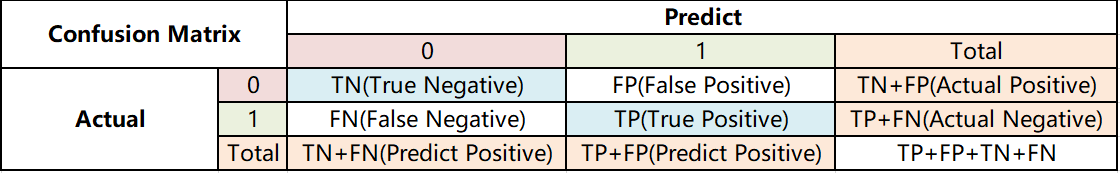
\includegraphics[width=\textwidth]{figures/指标.png}
  \caption{模型评估指标}
  \label{fig:zhibiao}
\end{figure}
\section{文本组织架构}
本文基于对近期研究热点音频特征建模技术,将其与目前健康检测领域的痛点相结合,并聚焦于目前一种常见的呼吸道疾病——哮喘,提出了一种基于音频特征建模的哮喘检测系统。该论文的总体组织结构如下:

第一章为绪论。本章简单介绍了当前健康检测领域的发展现状,并分析了当前健康检测领域的痛点和音频特征建模技术的优势。最后介绍了本论文的主要工作点。

第二章为理论基础。本章首先介绍音频特征建模工作的基础,然后介绍音频数据增强方法,并分析音频增强方法对实验结果的影响、最后介绍深度卷积网络VGG的基本原理,并简单分析利用VGG提取音频特征的原因。

第三章为系统设计。本章首先介绍本论文系统的整体架构,然后分模块介绍最重要的四个部分:咳嗽音频获取与筛选、咳嗽音频的数据增强、特征提取网络的架构以及特征分类网络的架构。

第四章为实验设计及其结果。本章介绍如何利用k-折交叉验证设计实验验证设计模型的有效性;并将结果进行分析说明

第五章为总结与展望。本章对本文的研究工作进行总结,分析了本文提出模型的优缺点。并在该课题下对本研究未来的方向提出了新的展望。
